% uklad dokumentu
	\documentclass{article}
	\usepackage{xparse}
	\usepackage[margin=1cm]{geometry}
    \usepackage{enumerate} 
	\frenchspacing
    \linespread{1.2}
    \setlength{\parindent}{0pt}

% jezyk polski
	\usepackage[polish]{babel}
	\usepackage[utf8]{inputenc}
	\usepackage{polski}
 
% pakiety matematyczne
    \let\lll\undefined
	\usepackage{amssymb}
    \usepackage{amsthm}
	\usepackage{amsmath}
	\usepackage{amsfonts}
	\usepackage{tikz}

% hiperlacza
	\usepackage{hyperref}
	\hypersetup{
		colorlinks,
		citecolor=black,
		filecolor=black,
		linkcolor=black,
		urlcolor=black
	}

% wstawianie zdjec
	\usepackage{graphicx} 
	\pagenumbering{gobble}
	

% podstawowe informacje
    \title{Algorytmy metaheurystyczne 3}
    \author{Paweł Cegieła, Wojciech Sęk}

\begin{document} 

\maketitle

\section{Rodzaje algorytmu}
Algorytm genetyczny można podzielić ze względu na dwie znaczące modyfikacje:
\begin{itemize}
\item algorytm może działać na jednej populacji lub na wielu populacjach żyjących na osobnych wyspach
\item algorytm może działać całkowicie sekwencyjnie lub wykonywać część obliczeń równolegle
\end{itemize}

\section{Parametry algorytmów}
Dla algorytmu sekwencyjnego z jedną populacją podajemy następujące parametry:
\begin{itemize}
\item $matrix$: macierz przechowująca odległości między miastami z problemu TSP
\item $gen\_rand$: wartość logiczna mówiąca, czy pierwsze pokolenie ma być całkowicie losowe czy przybliżone innymi metaheurystykami
\item $gen\_size$: liczność populacji na każdym etapie algorytmu
\item $elite\_num$: liczność elity, czyli najlepszych rozwiązań, które przeżywają i przechodzą do następnego pokolenia
\item $cross\_op$: wartość enumeratywna mówiąca o tym, jaki typ krzyżowania zostanie użyty w algorytmie. Możliwe wartości:
\begin{itemize}
\item 0 - HALF CROSSOVER: dziecko w każdym kroku generowania przyjmuje kolejne od jednego z rodziców miasto z prawdopodobieństwem 1/2, bierzemy najwcześniejsze miasto z rodzica, które nie występuje w dziecku
\item 1 - ORDER CROSSOVER: pół dziecka to podciąg rodzica, drugie pół to podciąg drugiego rodzica składający się z nieużytych wcześniej miast i zaczynający od miasta występującego na tym miejscu w pierwszym rodzicu
\item 2 - CYCLE CROSSOVER: bierzemy miasto z pierwszego rodzica, patrzymy na miasto pod danym indeksem w drugim rodzicu, idziemy do niego w pierwszym rodzicu, powtarzamy aż zamkniemy cykl. Resztę uzupełniamy drugim rodzicem.
\item 3 - PARTIALLY MAPPED CROSSOVER: na danym podciągu indeksów tworzymy mapę między rodzicami, następnie używamy pociągu z jednego rodzica i zmapowanych wartości z drugiego.
\end{itemize}
\item $swap\_change$: wartość logiczna decydująca o tym, czy w trakcie mutacji poruszamy się w sąsiedztwie $swap$ czy $reverse$
\item $size\_of\_tournament$: rozmiar turnieju przy losowaniu rodziców do tworzenia nowego pokolenia. Wartość ustawiona na 0 sprawia, że zamiast turnieju korzystamy z zasady ruletki, gdzie funkcja dopasowania jest odwrotnością wagi danej permutacji.
\item $mut\_chance$: prawdopodobieństwo, że dany osobnik zmutuje.
\item $max\_time$: ograniczenie czasowe, po którym algorytm kończy działanie. Wynik zwracany przez algorytm to najlepszy wynik znaleziony przed przekroczeniem limitu czasowego. 

\end{itemize}
Dla algorytmu wyspowego podajemy także:
\begin{itemize}
\item $isles\_num$: liczba wysp 
\item $migration\_freq$: liczba iteracji, które dzielą od siebie moment wymiany genetycznej między wyspami
\end{itemize}

W algorytmach urównoleglonych podaje się również parametr $num\_of\_threads$, który mówi o liczbie wątków.

\section{Teoretyczna złożoność}
Rozważmy złożoności poszczególnych etapów w algorytmie sekwencyjnym bez wysp. Niech $n$ to liczba miast, a $k$ to liczność pokolenia:
\begin{itemize}
\item \textbf{Wyznaczanie populacji początkowej}: w języku Rust losowanie permutacji ma złożoność $O(1)$, zatem losowa generacja osobników ma złożoność $O(k)$. Dla przybliżeń przez inne metaheurystyki co najwyżej $\frac{k}{4}$ jest przybliżone, w naszym przypadku dajemy jeden raz $2-OPT$ ze złożonością $O(n^3)$ i pozostałe to $nearest-neighbours$ od losowego miasta ze złożonością $O(n^2)$.
\item \textbf{Ewaluacja}: Obliczanie wartości danej permutacji ma złożoność $O(n)$, robimy to $k$ razy, zatem cały krok ma $O(kn)$.
\item \textbf{Selekcja}: Wybieramy $k$ rodziców. Przy ruletce wybór rodzica ma złożoność $O(1)$, przy turnieju $O(l)$, gdzie $l$ to rozmiar turnieju. Zatem $O(k)$ dla ruletki i $O(kl)$ dla turnieju.
\item \textbf{Krzyżowanie}: Każde z krzyżowań odbywa się w czasie liniowym względem długości permutacji, czyli $O(n)$, przy tworzeniu całej permutacji mamy $O(kn)$.
\item \textbf{Mutacja}: mutacja typu $swap$ ma złożoność $\Theta(1)$, a typu $reverse$ $\Theta(n)$. Mutacji wykonujemy $\Theta(pn)$, gdzie $p$ to prawdopodobieństwo mutacji. Zatem ta faza ma złożoność $\Theta(pn)$ lub $\Theta(pn^2)$. W worst case możemu wylosować wszystkie, więc odpowiednio złożoności są $O(n)$ i $O(n^2)$.
\end{itemize}
Ponadto w algorytmie wyspowym regularnie w niektórych iteracjach wymieniana jest informacja genetyczna ze złożonością $O(k^2)$ (każda wyspa wymienia się z każdą jakimś osobnikiem).

Podsumowując, w najgorszym przypadku:
\begin{itemize}
\item \textbf{Generacja początkowej populacji}: $$O(n^3+kn^2+k)=O((n+k)n^2)$$
\item \textbf{Właściwa iteracja:}
$$O(kn)+O(kl)+O(kn)+O(n^2)+O(k^2)=O(k(n+l+k)+n^2)$$
\end{itemize}
\section{Wykonane eksperymenty}

Strojenie algorytmu zostało wykonane na podstawie danych z TSPLIB. Wybrane zostały parametry, dla których algorytm najlepiej zachowywał się podczas testowania. Jeśli jeden z dwóch parametrów miał np. lepsze wyniki od drugiego dla jednych danych (np. dla mniejszych wielkości macierzy), a gorsze dla innych, wybierany był jeden z tych parametrów po przemyśleniu.

Po strojeniu zostały przeprowadzone eksperymenty porównujące algorytm w wersji oraz z parametrami wybranymi jako domyślne: z innymi wersjami algorytmu oraz z tabu search, a także z różnymi wartościami parametrów. Nie w każdym eksperymencie czy nie dla każdego typu macierzy domyślny algorytm okazał się najlepszy, natomiast strojenie pomogło nam znaleźć taki algorytm oraz parametry, które średnio zachowują się najlepiej.

\subsection{Porównanie wersji algorytmu genetycznego i tabu search}

\begin{center}
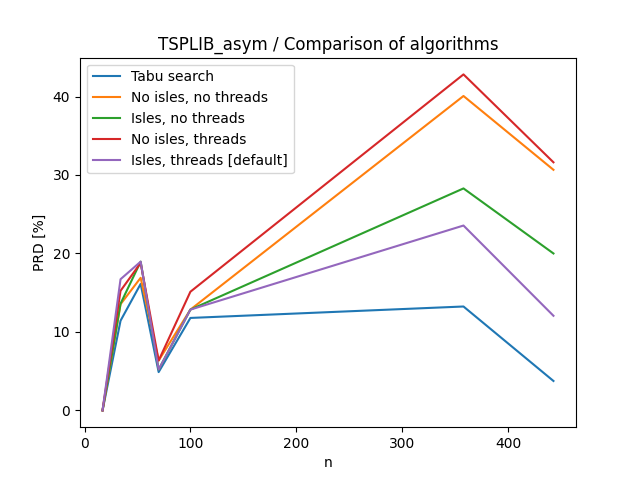
\includegraphics[width=\textwidth, 
                   height = 0.4\textheight, 
                   keepaspectratio]
                  {plots/tsplib_asym_1_comparison} 
\end{center}

\begin{center}
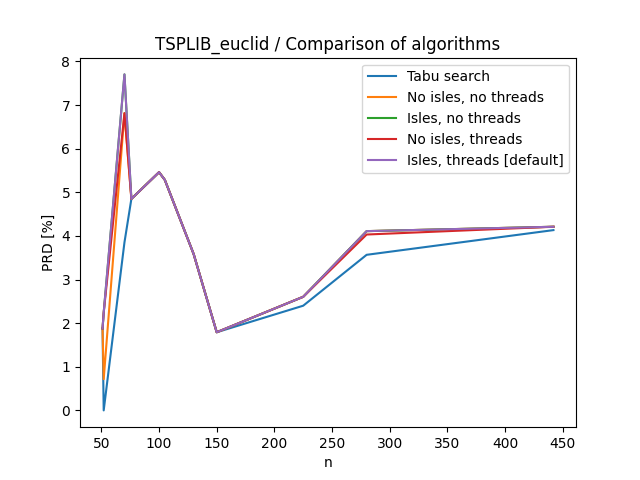
\includegraphics[width=\textwidth, 
                   height = 0.4\textheight, 
                   keepaspectratio]
                  {plots/tsplib_euclid_1_comparison} 
\end{center}

\begin{center}
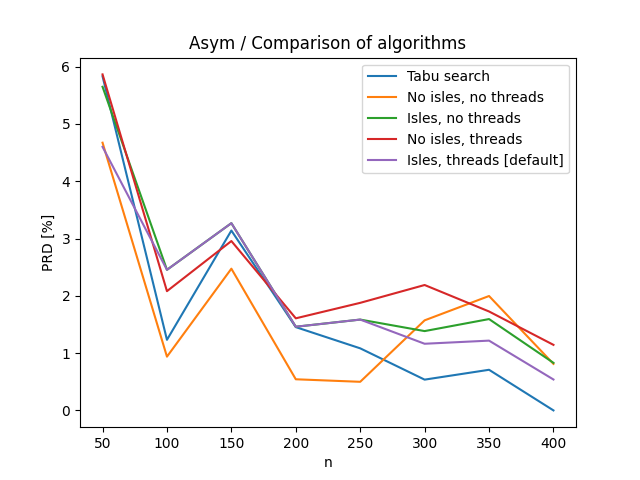
\includegraphics[width=\textwidth, 
                   height = 0.4\textheight, 
                   keepaspectratio]
                  {plots/asym_1_comparison} 
\end{center}

\begin{center}
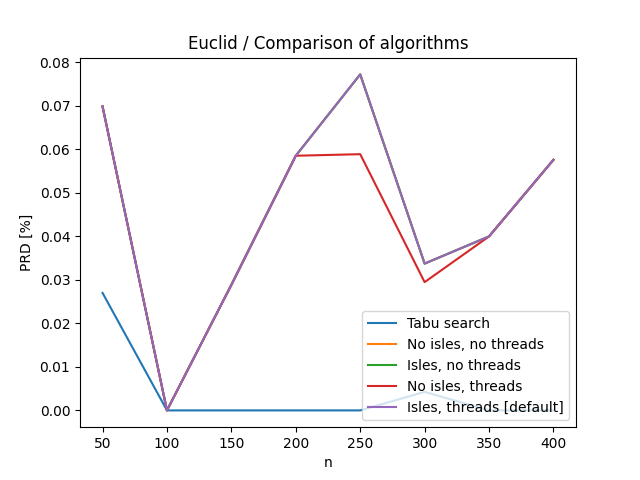
\includegraphics[width=\textwidth, 
                   height = 0.4\textheight, 
                   keepaspectratio]
                  {plots/euclid_1_comparison} 
\end{center}

\begin{center}
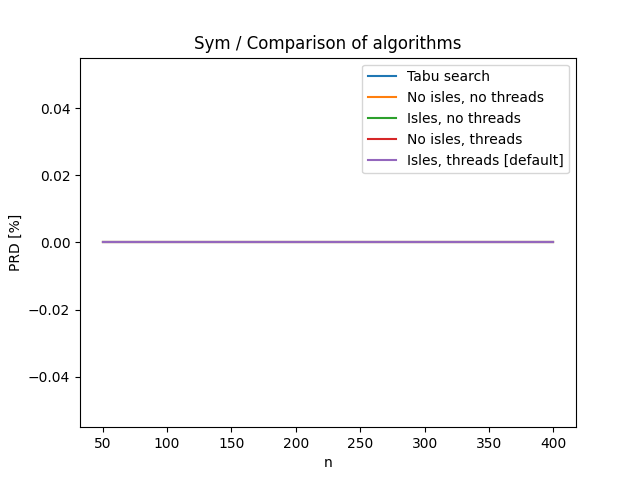
\includegraphics[width=\textwidth, 
                   height = 0.4\textheight, 
                   keepaspectratio]
                  {plots/sym_1_comparison} 
\end{center}


\subsection{Przybliżenie początkowe}

\begin{center}
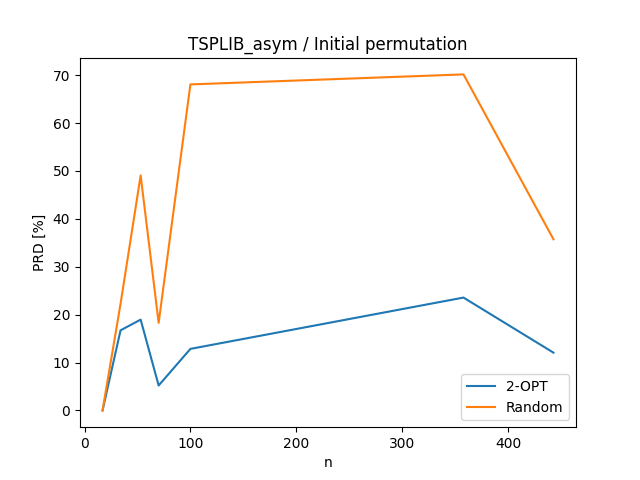
\includegraphics[width=\textwidth, 
                   height = 0.4\textheight, 
                   keepaspectratio]
                  {plots/tsplib_asym_2_gen_rand} 
\end{center}

\begin{center}
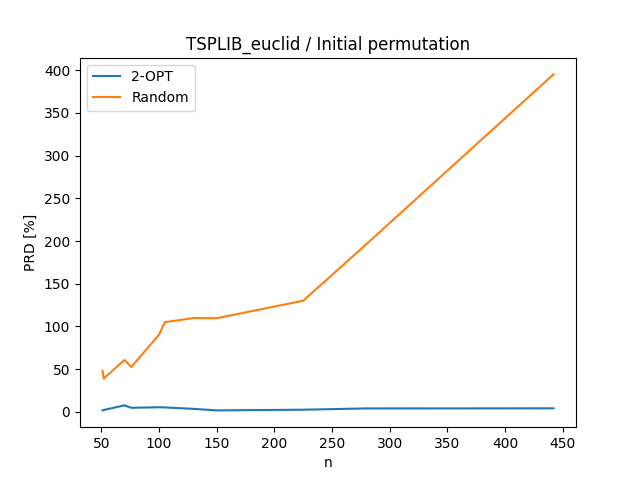
\includegraphics[width=\textwidth, 
                   height = 0.4\textheight, 
                   keepaspectratio]
                  {plots/tsplib_euclid_2_gen_rand} 
\end{center}

\begin{center}
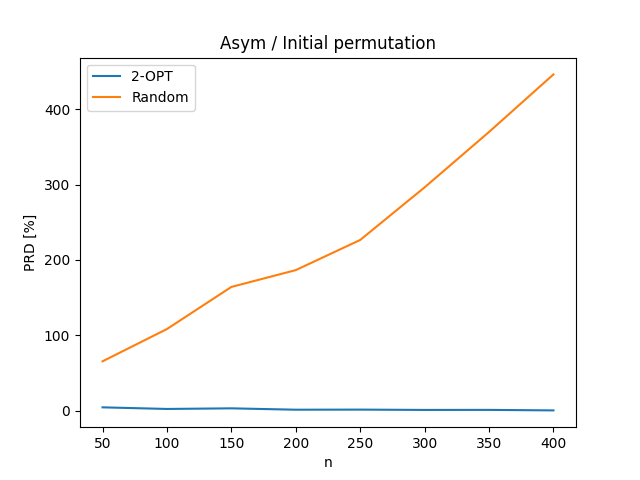
\includegraphics[width=\textwidth, 
                   height = 0.4\textheight, 
                   keepaspectratio]
                  {plots/asym_2_gen_rand} 
\end{center}

\begin{center}
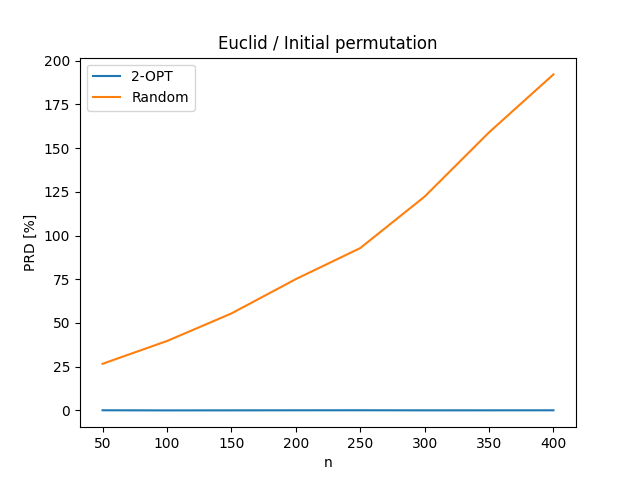
\includegraphics[width=\textwidth, 
                   height = 0.4\textheight, 
                   keepaspectratio]
                  {plots/euclid_2_gen_rand} 
\end{center}

\begin{center}
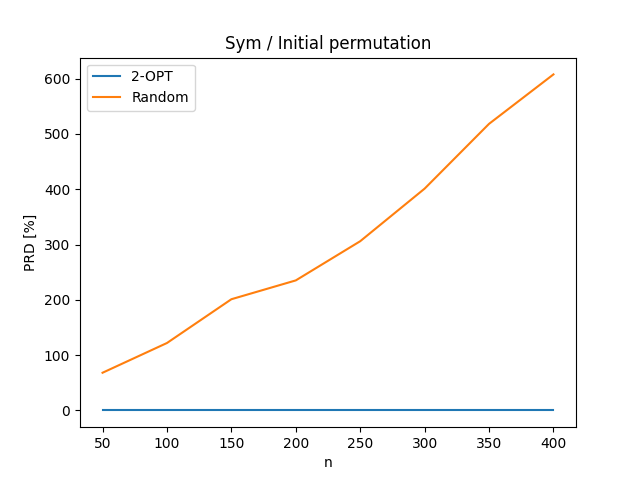
\includegraphics[width=\textwidth, 
                   height = 0.4\textheight, 
                   keepaspectratio]
                  {plots/sym_2_gen_rand} 
\end{center}


\subsection{Wielkość pokolenia}

\begin{center}
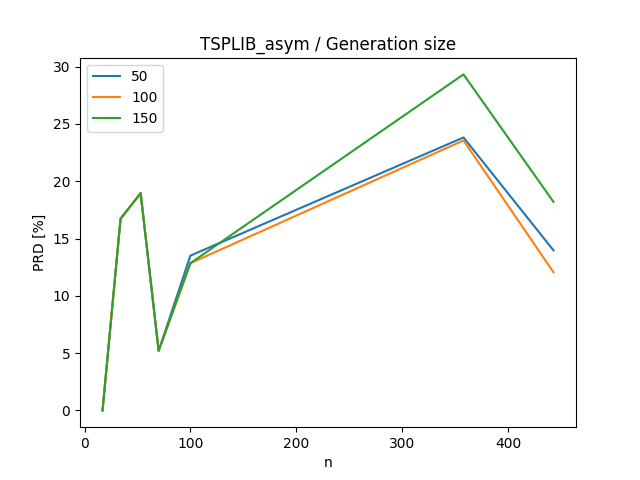
\includegraphics[width=\textwidth, 
                   height = 0.4\textheight, 
                   keepaspectratio]
                  {plots/tsplib_asym_3_generation_size} 
\end{center}

\begin{center}
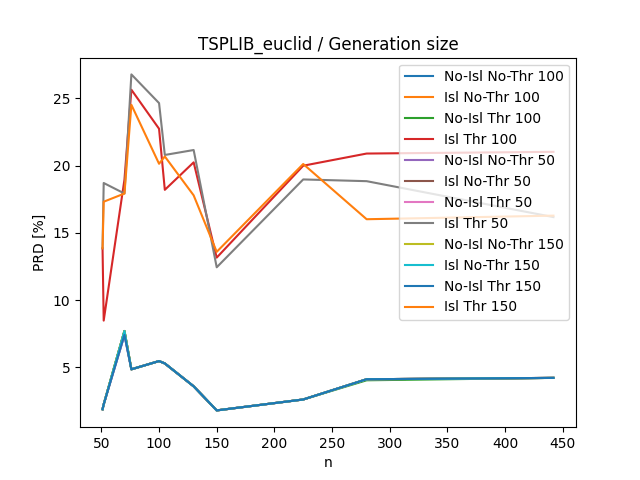
\includegraphics[width=\textwidth, 
                   height = 0.4\textheight, 
                   keepaspectratio]
                  {plots/tsplib_euclid_3_generation_size} 
\end{center}

\begin{center}
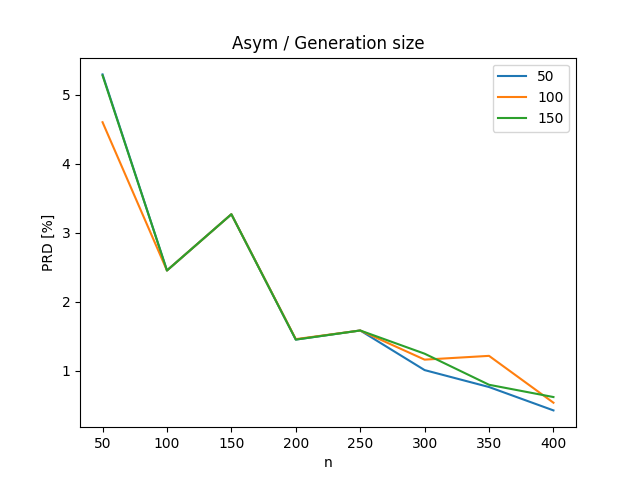
\includegraphics[width=\textwidth, 
                   height = 0.4\textheight, 
                   keepaspectratio]
                  {plots/asym_3_generation_size} 
\end{center}

\begin{center}
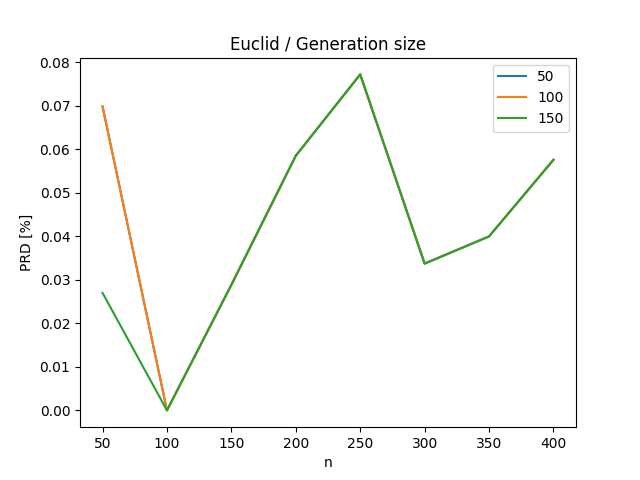
\includegraphics[width=\textwidth, 
                   height = 0.4\textheight, 
                   keepaspectratio]
                  {plots/euclid_3_generation_size} 
\end{center}

\begin{center}
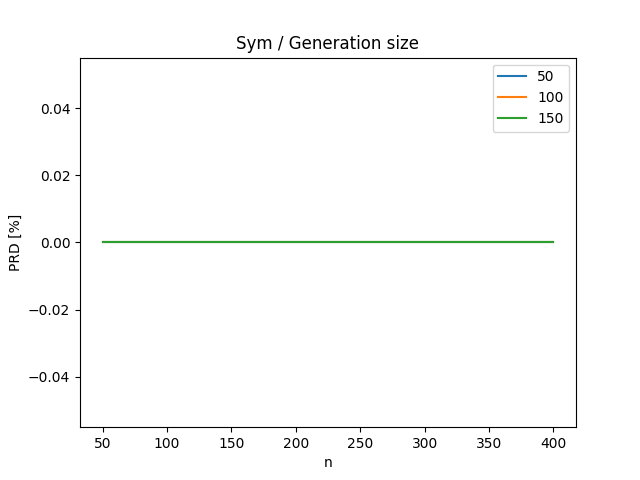
\includegraphics[width=\textwidth, 
                   height = 0.4\textheight, 
                   keepaspectratio]
                  {plots/sym_3_generation_size} 
\end{center}


\subsection{Wielkość elity}

\begin{center}
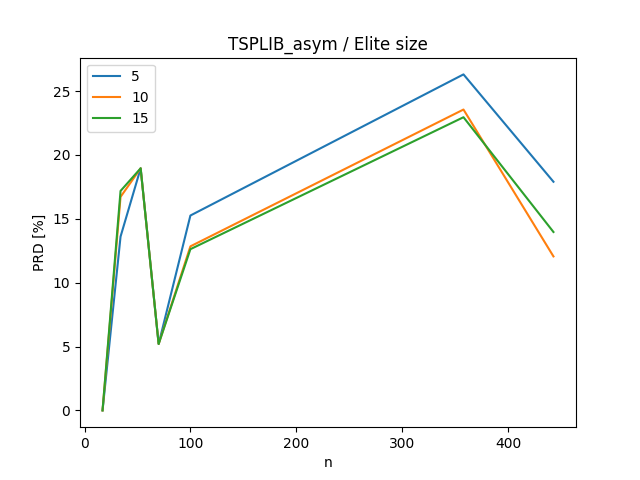
\includegraphics[width=\textwidth, 
                   height = 0.4\textheight, 
                   keepaspectratio]
                  {plots/tsplib_asym_4_elite_num} 
\end{center}

\begin{center}
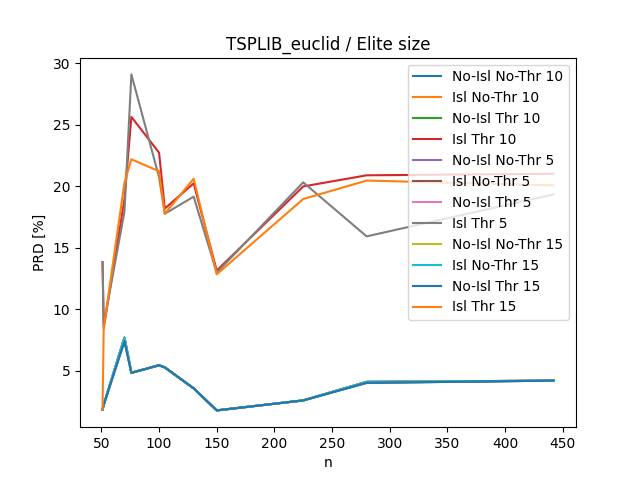
\includegraphics[width=\textwidth, 
                   height = 0.4\textheight, 
                   keepaspectratio]
                  {plots/tsplib_euclid_4_elite_num} 
\end{center}

\begin{center}
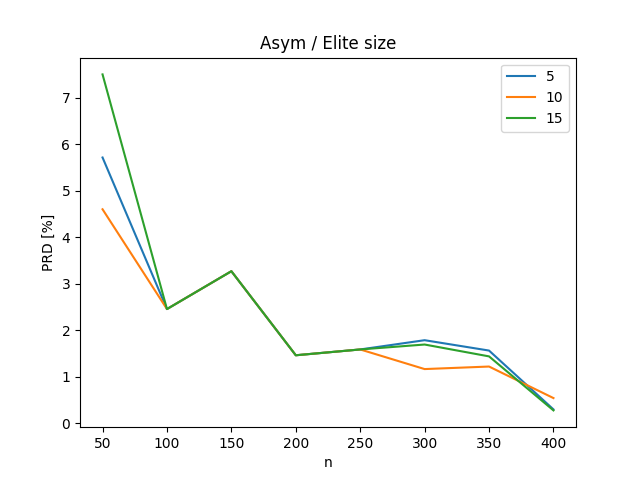
\includegraphics[width=\textwidth, 
                   height = 0.4\textheight, 
                   keepaspectratio]
                  {plots/asym_4_elite_num} 
\end{center}

\begin{center}
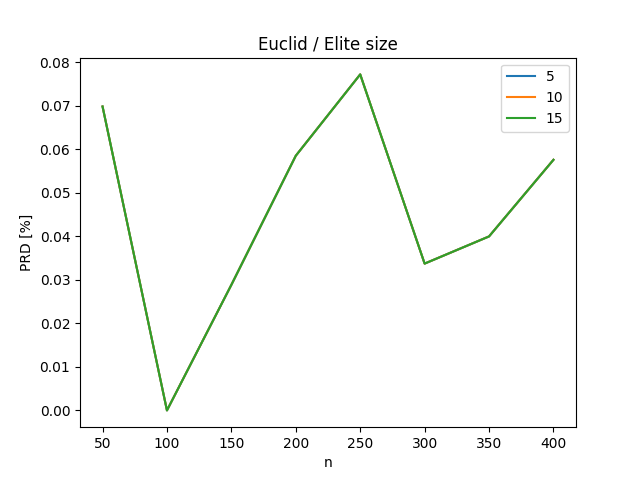
\includegraphics[width=\textwidth, 
                   height = 0.4\textheight, 
                   keepaspectratio]
                  {plots/euclid_4_elite_num} 
\end{center}

\begin{center}
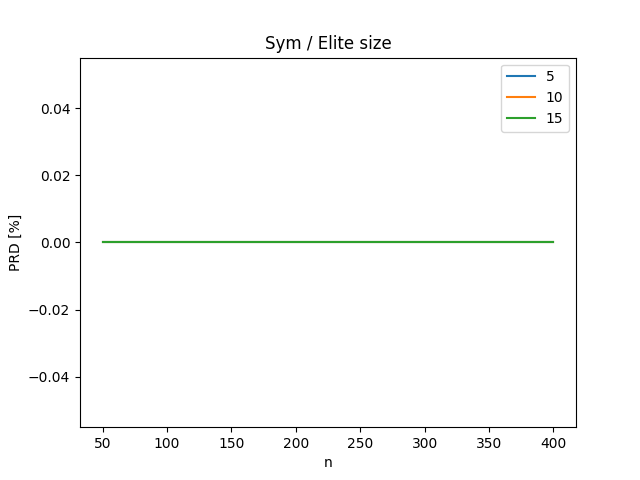
\includegraphics[width=\textwidth, 
                   height = 0.4\textheight, 
                   keepaspectratio]
                  {plots/sym_4_elite_num} 
\end{center}


\subsection{Krzyżowanie}

\begin{center}
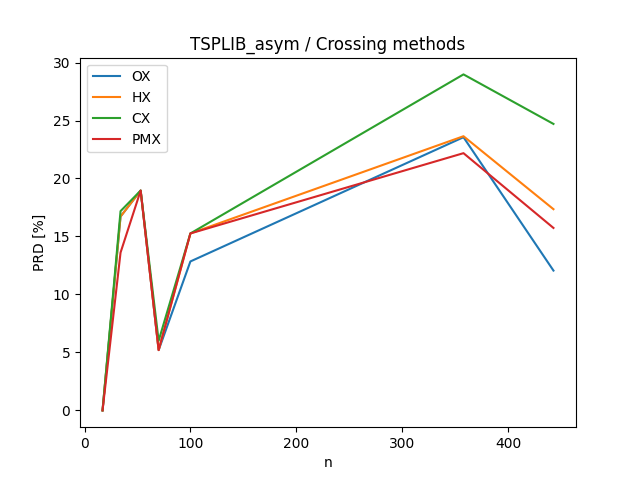
\includegraphics[width=\textwidth, 
                   height = 0.4\textheight, 
                   keepaspectratio]
                  {plots/tsplib_asym_5_crossing} 
\end{center}

\begin{center}
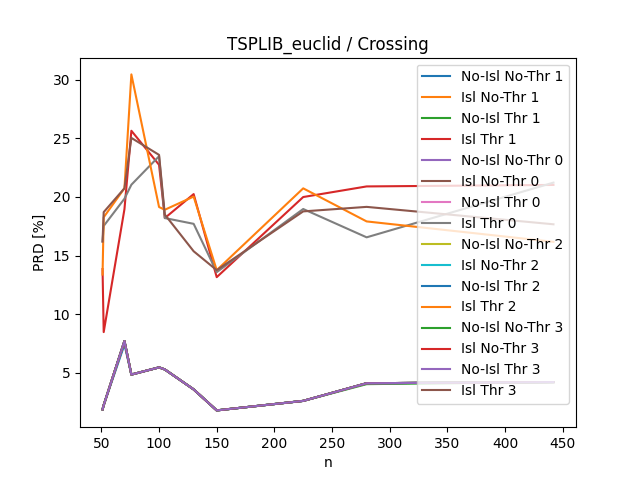
\includegraphics[width=\textwidth, 
                   height = 0.4\textheight, 
                   keepaspectratio]
                  {plots/tsplib_euclid_5_crossing} 
\end{center}

\begin{center}
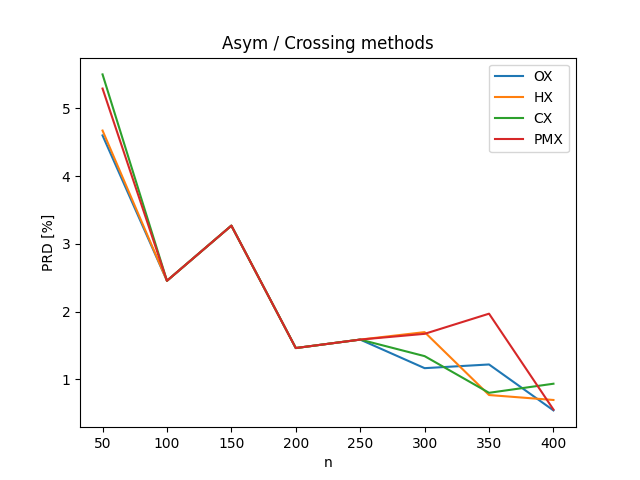
\includegraphics[width=\textwidth, 
                   height = 0.4\textheight, 
                   keepaspectratio]
                  {plots/asym_5_crossing} 
\end{center}

\begin{center}
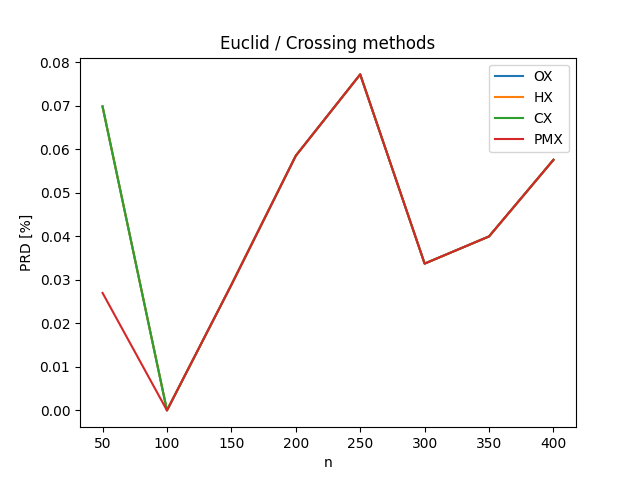
\includegraphics[width=\textwidth, 
                   height = 0.4\textheight, 
                   keepaspectratio]
                  {plots/euclid_5_crossing} 
\end{center}

\begin{center}
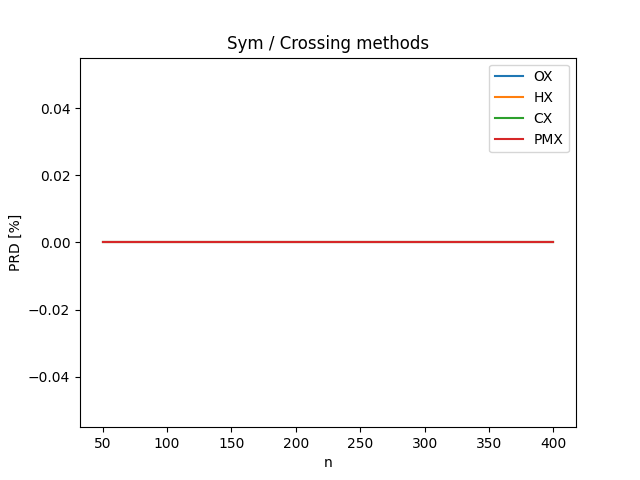
\includegraphics[width=\textwidth, 
                   height = 0.4\textheight, 
                   keepaspectratio]
                  {plots/sym_5_crossing} 
\end{center}


\subsection{Swap i inverse}

\begin{center}
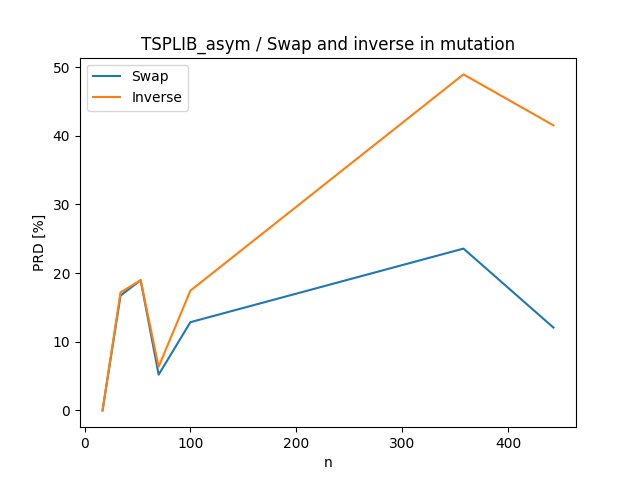
\includegraphics[width=\textwidth, 
                   height = 0.4\textheight, 
                   keepaspectratio]
                  {plots/tsplib_asym_6_swap_inverse} 
\end{center}

\begin{center}
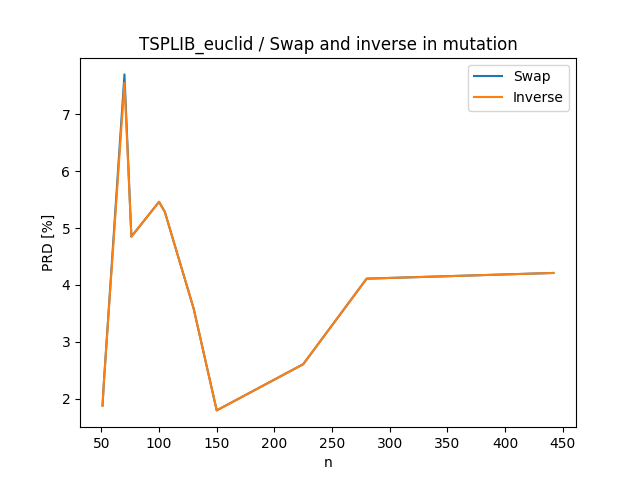
\includegraphics[width=\textwidth, 
                   height = 0.4\textheight, 
                   keepaspectratio]
                  {plots/tsplib_euclid_6_swap_inverse} 
\end{center}

\begin{center}
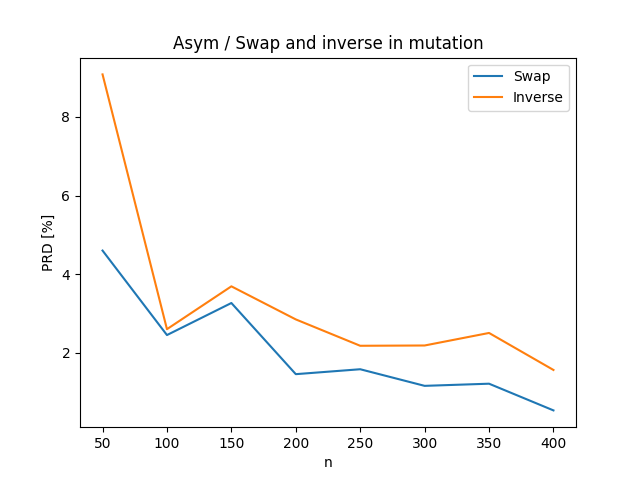
\includegraphics[width=\textwidth, 
                   height = 0.4\textheight, 
                   keepaspectratio]
                  {plots/asym_6_swap_inverse} 
\end{center}

\begin{center}
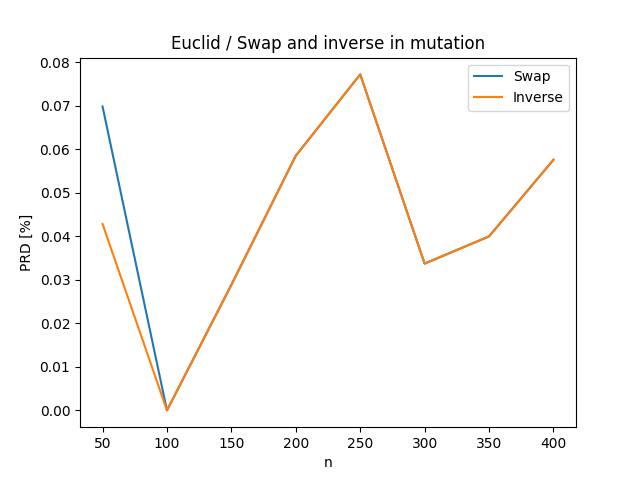
\includegraphics[width=\textwidth, 
                   height = 0.4\textheight, 
                   keepaspectratio]
                  {plots/euclid_6_swap_inverse} 
\end{center}

\begin{center}
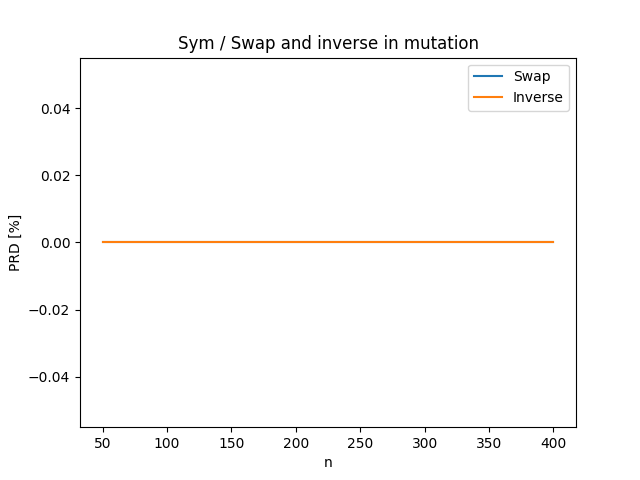
\includegraphics[width=\textwidth, 
                   height = 0.4\textheight, 
                   keepaspectratio]
                  {plots/sym_6_swap_inverse} 
\end{center}


\subsection{Turniej}

\begin{center}
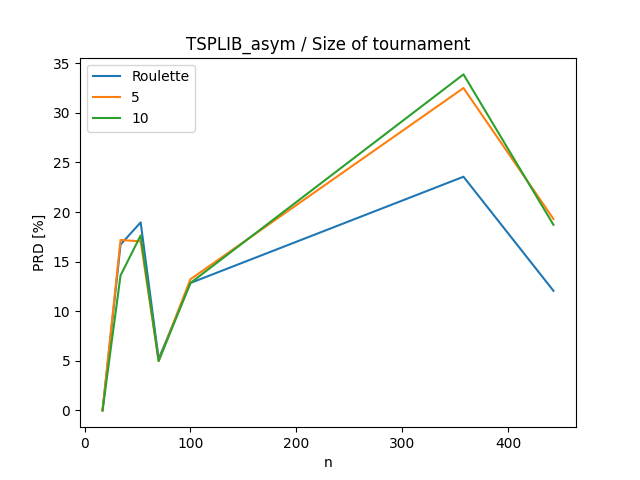
\includegraphics[width=\textwidth, 
                   height = 0.4\textheight, 
                   keepaspectratio]
                  {plots/tsplib_asym_7_tour} 
\end{center}

\begin{center}
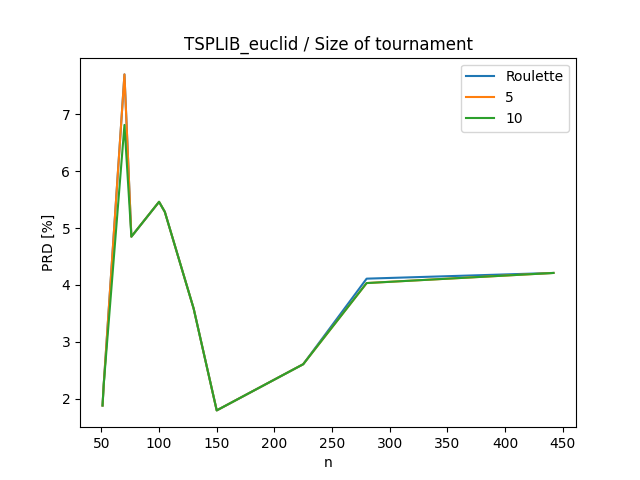
\includegraphics[width=\textwidth, 
                   height = 0.4\textheight, 
                   keepaspectratio]
                  {plots/tsplib_euclid_7_tour} 
\end{center}

\begin{center}
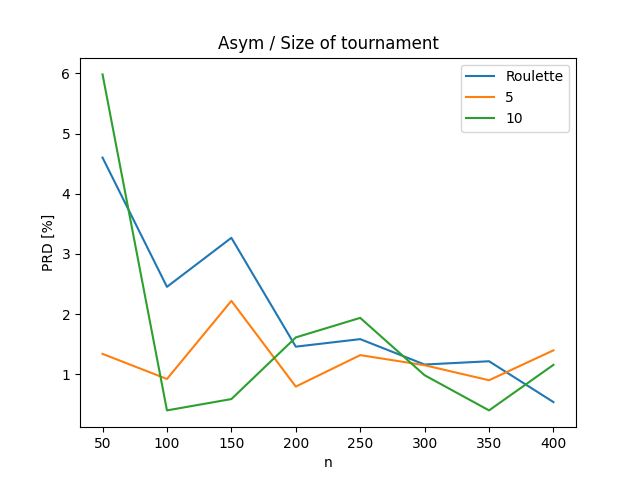
\includegraphics[width=\textwidth, 
                   height = 0.4\textheight, 
                   keepaspectratio]
                  {plots/asym_7_tour} 
\end{center}

\begin{center}
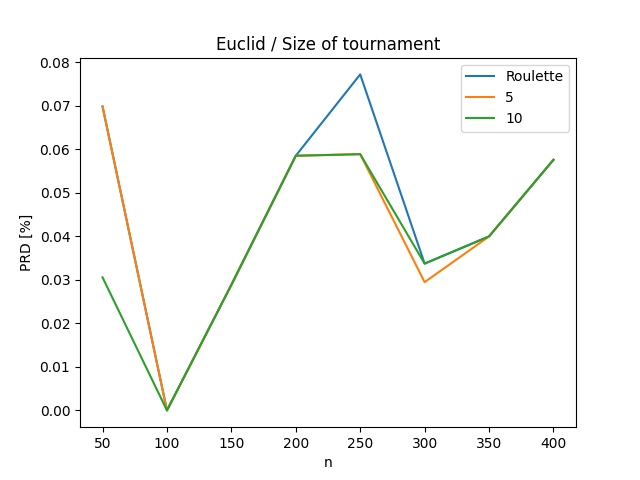
\includegraphics[width=\textwidth, 
                   height = 0.4\textheight, 
                   keepaspectratio]
                  {plots/euclid_7_tour} 
\end{center}

\begin{center}
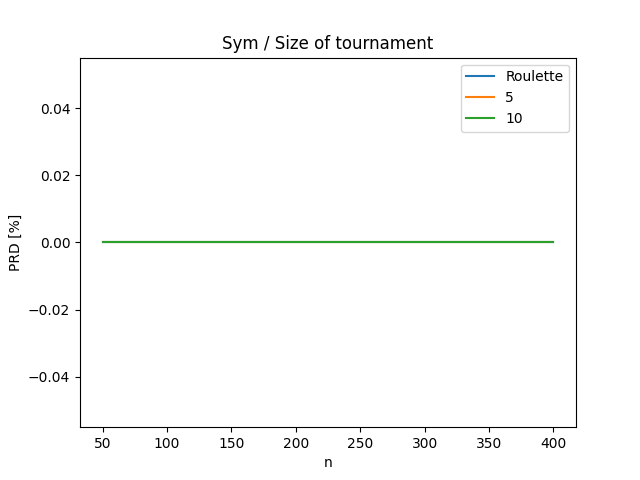
\includegraphics[width=\textwidth, 
                   height = 0.4\textheight, 
                   keepaspectratio]
                  {plots/sym_7_tour} 
\end{center}


\subsection{Szansa mutacji}

\begin{center}
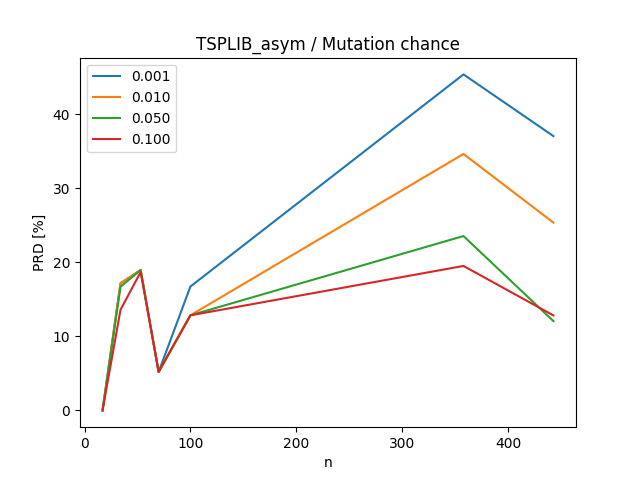
\includegraphics[width=\textwidth, 
                   height = 0.4\textheight, 
                   keepaspectratio]
                  {plots/tsplib_asym_8_mut_chance} 
\end{center}

\begin{center}
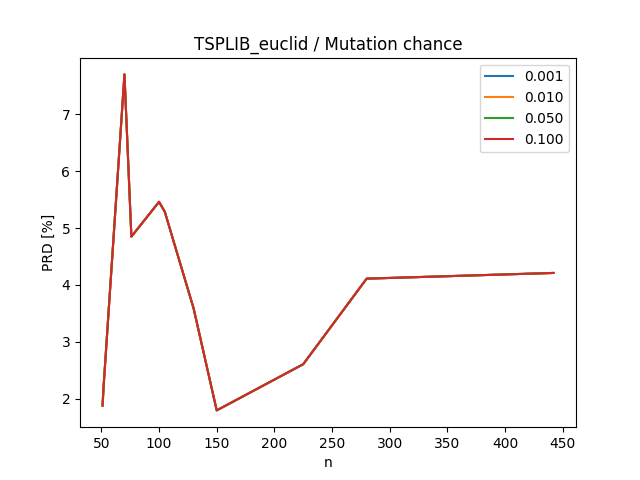
\includegraphics[width=\textwidth, 
                   height = 0.4\textheight, 
                   keepaspectratio]
                  {plots/tsplib_euclid_8_mut_chance} 
\end{center}

\begin{center}
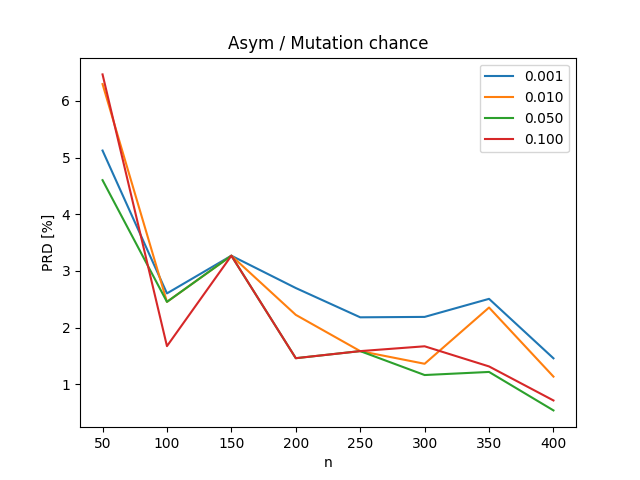
\includegraphics[width=\textwidth, 
                   height = 0.4\textheight, 
                   keepaspectratio]
                  {plots/asym_8_mut_chance} 
\end{center}

\begin{center}
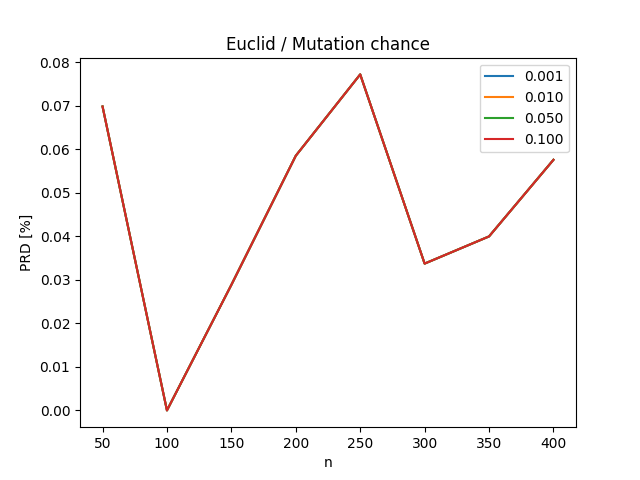
\includegraphics[width=\textwidth, 
                   height = 0.4\textheight, 
                   keepaspectratio]
                  {plots/euclid_8_mut_chance} 
\end{center}

\begin{center}
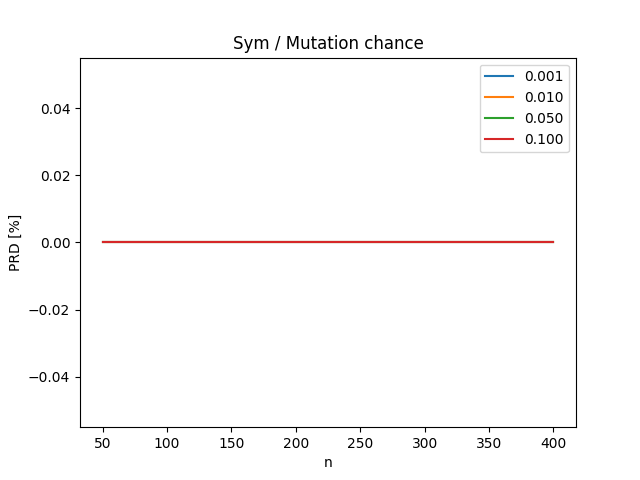
\includegraphics[width=\textwidth, 
                   height = 0.4\textheight, 
                   keepaspectratio]
                  {plots/sym_8_mut_chance} 
\end{center}


\subsection{Maksymalny czas}

\begin{center}
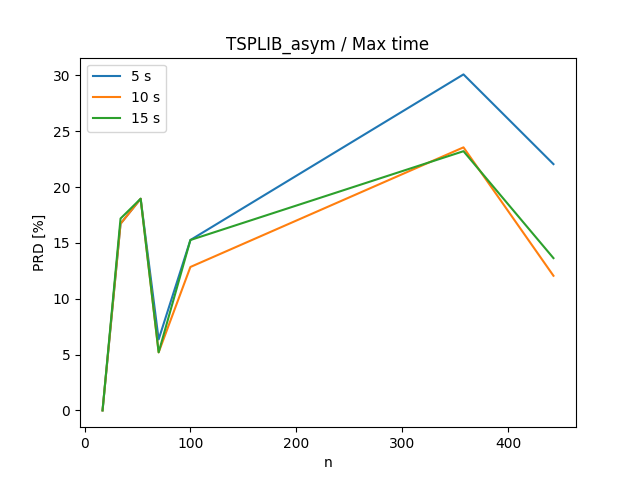
\includegraphics[width=\textwidth, 
                   height = 0.4\textheight, 
                   keepaspectratio]
                  {plots/tsplib_asym_9_max_time} 
\end{center}

\begin{center}
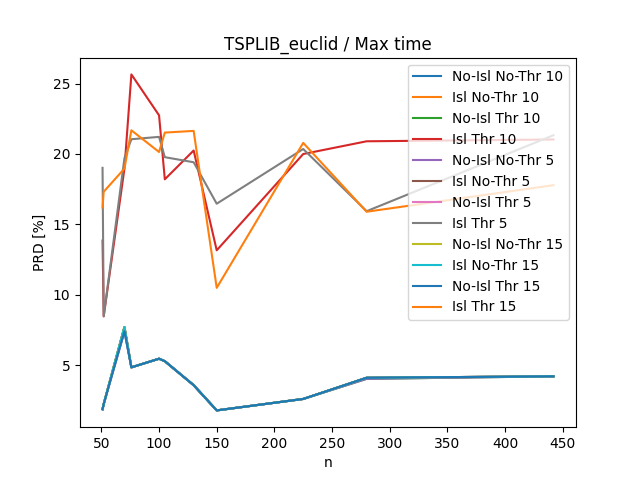
\includegraphics[width=\textwidth, 
                   height = 0.4\textheight, 
                   keepaspectratio]
                  {plots/tsplib_euclid_9_max_time} 
\end{center}

\begin{center}
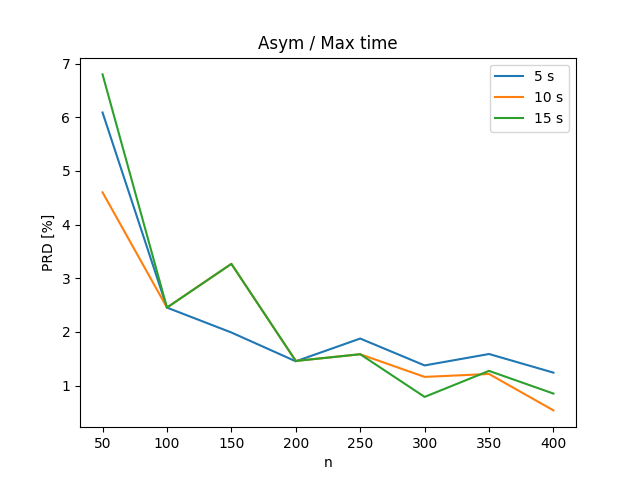
\includegraphics[width=\textwidth, 
                   height = 0.4\textheight, 
                   keepaspectratio]
                  {plots/asym_9_max_time} 
\end{center}

\begin{center}
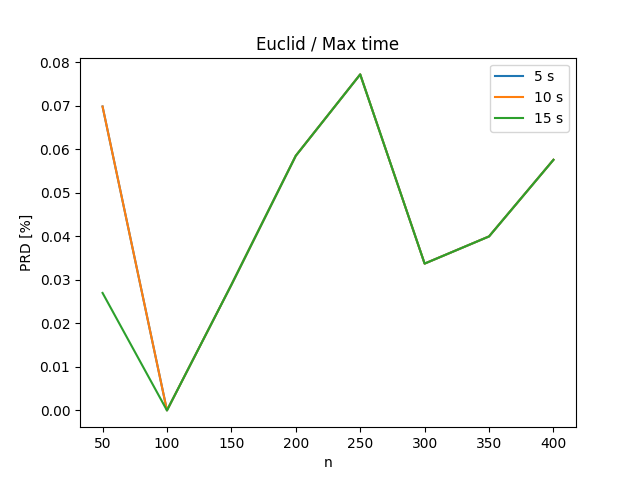
\includegraphics[width=\textwidth, 
                   height = 0.4\textheight, 
                   keepaspectratio]
                  {plots/euclid_9_max_time} 
\end{center}

\begin{center}
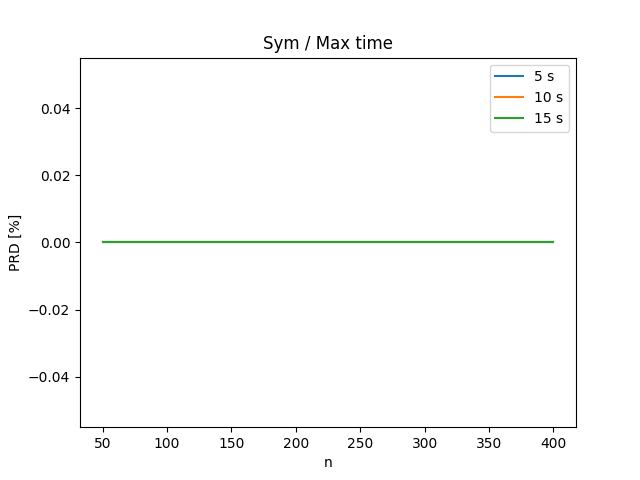
\includegraphics[width=\textwidth, 
                   height = 0.4\textheight, 
                   keepaspectratio]
                  {plots/sym_9_max_time} 
\end{center}


\subsection{Liczba wysp}

\begin{center}
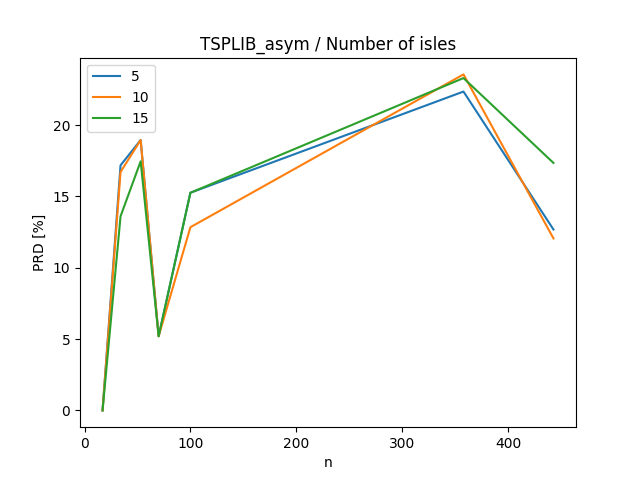
\includegraphics[width=\textwidth, 
                   height = 0.4\textheight, 
                   keepaspectratio]
                  {plots/tsplib_asym_10_isles} 
\end{center}

\begin{center}
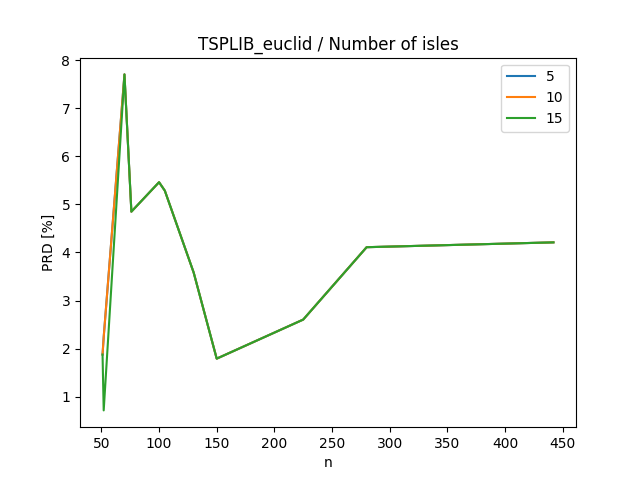
\includegraphics[width=\textwidth, 
                   height = 0.4\textheight, 
                   keepaspectratio]
                  {plots/tsplib_euclid_10_isles} 
\end{center}

\begin{center}
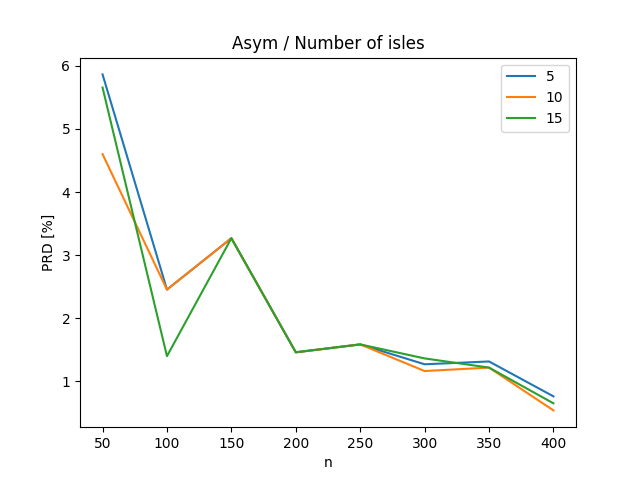
\includegraphics[width=\textwidth, 
                   height = 0.4\textheight, 
                   keepaspectratio]
                  {plots/asym_10_isles} 
\end{center}

\begin{center}
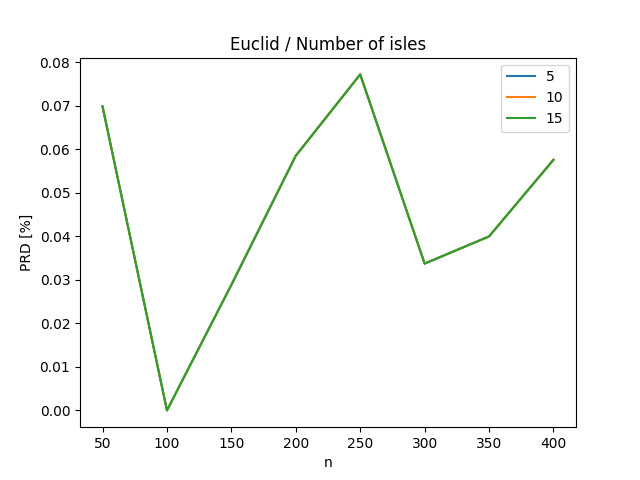
\includegraphics[width=\textwidth, 
                   height = 0.4\textheight, 
                   keepaspectratio]
                  {plots/euclid_10_isles} 
\end{center}

\begin{center}
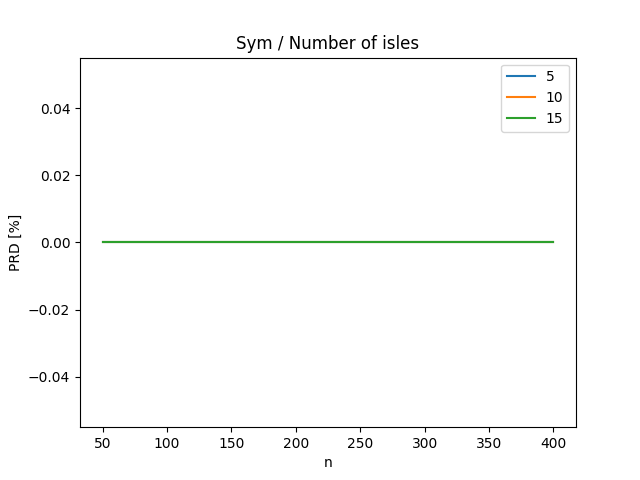
\includegraphics[width=\textwidth, 
                   height = 0.4\textheight, 
                   keepaspectratio]
                  {plots/sym_10_isles} 
\end{center}


\subsection{Częstotliwość migracji}

\begin{center}
\includegraphics[width=\textwidth, 
                   height = 0.4\textheight, 
                   keepaspectratio]
                  {plots/tsplib_asym_11_migration_freq} 
\end{center}

\begin{center}
\includegraphics[width=\textwidth, 
                   height = 0.4\textheight, 
                   keepaspectratio]
                  {plots/tsplib_euclid_11_migration_freq} 
\end{center}

\begin{center}
\includegraphics[width=\textwidth, 
                   height = 0.4\textheight, 
                   keepaspectratio]
                  {plots/asym_11_migration_freq} 
\end{center}

\begin{center}
\includegraphics[width=\textwidth, 
                   height = 0.4\textheight, 
                   keepaspectratio]
                  {plots/euclid_11_migration_freq} 
\end{center}

\begin{center}
\includegraphics[width=\textwidth, 
                   height = 0.4\textheight, 
                   keepaspectratio]
                  {plots/sym_11_migration_freq} 
\end{center}


\subsection{Liczba wątków}

\begin{center}
\includegraphics[width=\textwidth, 
                   height = 0.4\textheight, 
                   keepaspectratio]
                  {plots/tsplib_asym_12_num_of_threads} 
\end{center}

\begin{center}
\includegraphics[width=\textwidth, 
                   height = 0.4\textheight, 
                   keepaspectratio]
                  {plots/tsplib_euclid_12_num_of_threads} 
\end{center}

\begin{center}
\includegraphics[width=\textwidth, 
                   height = 0.4\textheight, 
                   keepaspectratio]
                  {plots/asym_12_num_of_threads} 
\end{center}

\begin{center}
\includegraphics[width=\textwidth, 
                   height = 0.4\textheight, 
                   keepaspectratio]
                  {plots/euclid_12_num_of_threads} 
\end{center}

\begin{center}
\includegraphics[width=\textwidth, 
                   height = 0.4\textheight, 
                   keepaspectratio]
                  {plots/sym_12_num_of_threads} 
\end{center}



\section{Obserwacje i wnioski}
\begin{itemize}
\item Obserwacje i wnioski - do zrobienia
\end{itemize}

\end{document}